
%%%%%%%%%%%%%%%%%%%%%%% file typeinst.tex %%%%%%%%%%%%%%%%%%%%%%%%%
%
% This is the LaTeX source for the instructions to authors using
% the LaTeX document class 'llncs.cls' for contributions to
% the Lecture Notes in Computer Sciences series.
% http://www.springer.com/lncs       Springer Heidelberg 2006/05/04
%
% It may be used as a template for your own input - copy it
% to a new file with a new name and use it as the basis
% for your article.
%
% NB: the document class 'llncs' has its own and detailed documentation, see
% ftp://ftp.springer.de/data/pubftp/pub/tex/latex/llncs/latex2e/llncsdoc.pdf
%
%%%%%%%%%%%%%%%%%%%%%%%%%%%%%%%%%%%%%%%%%%%%%%%%%%%%%%%%%%%%%%%%%%%


\documentclass[runningheads,a4paper]{llncs}

\usepackage[utf8]{inputenc}
\usepackage[T1]{fontenc}
\usepackage{chngpage}

\usepackage{amssymb}
\setcounter{tocdepth}{3}
\usepackage{graphicx}
\usepackage{wrapfig}

\usepackage{url}
\newcommand{\keywords}[1]{\par\addvspace\baselineskip
\noindent\keywordname\enspace\ignorespaces#1}


\usepackage{hyperref}
\usepackage{listings}
%\usepackage[scaled]{luximono}


%\usepackage{natbib}

% ----- begin macros

\lstdefinelanguage{Scala}%
{morekeywords={abstract,%
  case,catch,char,class,%
  def,else,extends,final,for,%
  if,import,implicit,%
  match,module,%
  new,null,%
  object,override,%
  package,private,protected,public,%
  for,public,return,super,%
  this,throw,trait,try,type,%
  val,var,%
  with,%
  yield,%
  lazy%
  },%
  sensitive,%
  morecomment=[l]//,%
  morecomment=[s]{/*}{*/},%
  morestring=[b]",%
  morestring=[b]',%
  showstringspaces=false%
}[keywords,comments,strings]%

\lstdefinelanguage{JavaScript}%
{morekeywords={for, var, attributes, class, classend, do, else, empty, endif, endwhile, fail, function,
functionend, if, implements, in, inherit, inout, not, of, operations, out, return,
then, types, while, use},%
  sensitive,%
  morecomment=[l]//,%
  morecomment=[s]{/*}{*/},%
  morestring=[b]",%
  morestring=[b]',%
  showstringspaces=false%
}[keywords,comments,strings]%

\lstset{language=Scala,%
  mathescape=false,%
%  columns=[c]fixed,%
  aboveskip=\smallskipamount,
  belowskip=\smallskipamount,
%  basewidth={0.5em, 0.4em},%
  basicstyle=\ttfamily\small,%
  keywordstyle=\bfseries%\sffamily\bfseries,%
%  keywordstyle=\sffamily\bfseries,%
%  xleftmargin=0.5cm
}

\newcommand{\commentstyle}[1]{\slseries{#1}}
\newcommand{\keywordstyle}[1]{\bfseries{#1}}

\lstnewenvironment{slisting}{\lstset{language=Scala}}{}

\newcommand{\code}[1]{\lstinline[language=Scala,columns=fixed,basicstyle=\ttfamily\small]|#1|}

\def\changemargin#1#2{\list{}{\rightmargin#2\leftmargin#1}\item[]}
\let\endchangemargin=\endlist

%\setlength{\columnseprule}{0.25pt}

%\renewcommand{\note}[1]{$\spadesuit$ \textbf{#1} $\clubsuit$}


%\newcommand{\comment}[1]{}


\begin{document}

\mainmatter  % start of an individual contribution

\title{JavaScript as an Embedded DSL}
% a short form should be given in case it is too long for the running head
%\titlerunning{}

% the name(s) of the author(s) follow(s) next
%
% NB: Chinese authors should write their first names(s) in front of
% their surnames. This ensures that the names appear correctly in
% the running heads and the author index.
%
\author{Grzegorz Kossakowski \and Nada Amin \and Tiark Rompf \and Martin Odersky}
%
\authorrunning{JavaScript as an Embedded DSL}
% (feature abused for this document to repeat the title also on left hand pages)

% the affiliations are given next; don't give your e-mail address
% unless you accept that it will be published
\institute{Ecole Polytechnique F\'ed\'erale de Lausanne (EPFL)\\
\email{\texttt{\{first.last\}@epfl.ch}}}
%\mailsa\\
%\mailsb\\
%\url{http://lamp.epfl.ch}}

%
% NB: a more complex sample for affiliations and the mapping to the
% corresponding authors can be found in the file "llncs.dem"
% (search for the string "\mainmatter" where a contribution starts).
% "llncs.dem" accompanies the document class "llncs.cls".
%

%\toctitle{}
%\tocauthor{}
\maketitle


\begin{abstract}
% =>70 & <=150 words

Developing rich web applications requires mastering different
environments on the client and server sides. While there is
considerable choice on the server-side, the client-side is tied to
JavaScript, which poses considerable software engineering challenges,
such as moving or sharing pieces of code between the environments. We
embed JavaScript as a DSL in Scala, using Lightweight Modular Staging.
DSL code can be compiled to JavaScript or executed as part of the
server application. We use features of the host language to make
client-side programming safer and more convenient. We use gradual
typing to interface typed DSL programs with existing JavaScript APIs.
We exploit a selective CPS transform already available in the host
language to provide a compelling abstraction over asynchronous
callback-driven programming in our DSL.

\keywords{JavaScript, Scala, DSL, programming languages}
\end{abstract}

\section{Introduction}

Developing rich web applications requires mastering a heterogeneous environment: though the server-side can be implemented in any language, on the client-side, the choice is limited to JavaScript. The trend towards alternative approaches to client-side programming (as embodied by CoffeeScript~\cite{coffeescript}, Dart~\cite{dart} \& GWT~\cite{gwt}) shows the need for more options on the client-side. How do we bring advances in programming languages to client-side programming?

One challenge in developing a large code base in JavaScript is the lack of static typing, as types are helpful for maintenance, refactoring, and reasoning about correctness. Furthermore, there is a need for more abstraction and modularity. ``Inversion of control'' in asynchronous callback-driven programming leads to code with control structures that are difficult to reason about. A challenge is to introduce helpful abstractions without a big hit on performance and/or code size. Communication between the server side and the client side aggravates the impedance mismatch: in particular, data validation logic needs to be duplicated on the client-side for interactivity and on the server-side for security.

% Motivation for our approach vs other approaches

There are three widely known approaches for addressing the challenges outlined above. One is to create a standalone language or DSL that is compiled to JavaScript and provides different abstractions compared to JavaScript. Examples include WebDSL~\cite{webdsl}, Links~\cite{links,links-form} and Dart~\cite{dart}. However, this approach usually requires a lot of effort in terms of language and compiler design, and tooling support, although WebDSL leverages Spoofax~\cite{spoofax} to alleviate this effort. Furthermore, it is not always clear how these languages interact with other languages on the server-side or with the existing JavaScript ecosystem on the client-side.

Another approach is to start with an existing language like Java, Scala or Clojure and compile it to JavaScript. Examples include GWT~\cite{gwt}, Scala+GWT~\cite{scala-gwt} and Clojurescript~\cite{clojurescript}. This approach addresses the problem of impedance mismatch between client and server programming but comes with its own set of challenges. In particular, compiling Scala code to JavaScript requires compiling Scala's standard library to JavaScript as any non-trivial Scala program uses Scala collections. This leads to not taking full advantage of libraries and abstractions provided by the target platform which results in big code size and suboptimal performance of Scala applications compiled to JavaScript. For example, a map keyed by strings would be implemented natively in JavaScript as an object literal, while, in Scala, one would likely use the hash map from the standard library, causing it to be compiled to and emulated in JavaScript. Moreover, both approaches tend to not accommodate very well to different API design and programming styles seen in many existing JavaScript libraries. The F\# Web Tools~\cite{tomasp-fsharp} is another example of starting with an existing language, F\#, and compiling it to both the client and the server sides. This work has similar goals to ours but the underlying techniques are very different (explicit quotations vs LMS, monads vs cps). A drawback of this second approach is that the whole starting language needs to be translated to JavaScript: there is no easy or modular way to limit the scope of the source language.

A third approach is to design a language than is a thin layer on top of JavaScript but provides some new features. A prime example of this idea is CoffeeScript~\cite{coffeescript}. This approach makes it easy to integrate with existing JavaScript libraries but does not solve the impedance mismatch problem. In addition, it typically does not give rise to new abstractions addressing problems seen in callback-driven programming style, though some JavaScript libraries such as Flapjax~\cite{flapjax} and Arrowlets~\cite{arrowlets} are specifically designed for this purpose.

We present a different approach, based on Lightweight Modular Staging
(LMS)~\cite{lms}, that aims to incorporate good ideas from all the
approaches presented above but at the same time tries to avoid their
described shortcomings. LMS is a technique for embedding DSLs as
libraries into a host language such as Scala, while enabling
domain-specific compilation / code-generation. The program is split
into two stages: the first stage is a program generator that, when
run, produces the second stage program. Whether an expression belongs
to the first or second stage is decided by its type. Expressions
belonging to the second stage, also called ``staged expressions'',
have type \code{Rep[T]} in the first stage when yielding a computation
of type \code{T} in the second stage. Expressions evaluated in the
first stage become constants at the second stage. Other approaches to
staging include MetaML~\cite{metaml}, LISP quasiquotations, and
binding-time analysis in partial evaluation. Previous work has
established LMS as a pragmatic approach to runtime code generation and
compiled DSLs. In particular, the Delite
framework~\cite{brown11dsl,rompf11dsl,ppopp11delite} uses this
approach to provide an extensible suite of high-performance DSLs
targeting heterogeneous parallel platforms (with options to generate
code to Scala, C and Cuda)~\cite{lee11dsl}, for domains such as
machine learning~\cite{icml11optiml}, numeric array
processing~\cite{ureche12} and mesh-based partial differential
equation solvers~\cite{hassan10virtualization}. LMS has also been used
to generate SQL queries~\cite{siq}.

%Two widely used approaches to tackle these challenges is to create a new language which targets JavaScript (such as WebDSL) or to compile an existing language to JavaScript (such as GWT). These approaches make it difficult to inter-operate with existing JavaScript libraries. One could think of compiling Scala to JavaScript, but programming in Scala involves using the standard library. A naive translation of the Scala standard library to JavaScript might not Translating existing libraries in the source language to JavaScript

% WebDSL -> issue with integrating existing JS libraries
% compiling an existing language to JS -> 

% programmable code generator

We propose to embed JavaScript as a DSL in a host language.\footnote{Surely, the embedded language is not exactly JavaScript: it naturally is a subset of Scala, the host language. However, it is quite close to JavaScript: often one can take snippets of JavaScript code and use them in the DSL with minor syntactic tweaking (as demonstrated by the Snowflake example described in section \ref{sec:trivial-embedding}).} Through LMS, we tackle the challenges outlined above with minimal effort, as most of the work is off-loaded to the host language. In particular, we make the following contributions:
\begin{itemize}
\item Our DSL is statically typed through the host language, yet supports gradual typing notably for incorporating external JavaScript libraries and APIs (section~\ref{sec:typing}).
\item In addition to generating JavaScript code, our DSL can be executed directly in the host language, allowing code to be shared between client and server (section~\ref{sec:trivial-embedding}).
\item We use advanced object-oriented techniques to achieve modularity in our DSL: each language primitive and API is defined in a separate module (section~\ref{sec:modularity}).
\item Our DSL supports typed object literals and class-based objects. The translations to JavaScript are lightweight and intuitive: the object literals translate to JSON-like object literals and the class-based objects to JavaScript constructor-based objects (section~\ref{sec:reification}).
\item With minimal effort, we exploit the selective CPS transform already existing in the host language to provide a compelling abstraction over asynchronous callback-driven programming in our DSL (section~\ref{sec:cps}). This case-study demonstrates the fruitfulness of re-using host language features to enhance our embedded DSL. A novel insight is that CPS transforming a program generator allows it to generate code that is in CPS.
\end{itemize}

In section~\ref{sec:eval}, we describe our experience in using the DSL, and conclude in section~\ref{sec:conclusion}.

The present work extends both the range of virtualizable language features and the LMS framework, which is beneficial to future DSL efforts taking the JavaScript work as a case study. Previous LMS embeddings had to define each operation explicitly (like in section~\ref{sec:defineDslComponent}). This paper contributes lifting of whole traits or classes (through the \code{repProxy} mechanism described and used in sections~\ref{sec:typedApis}\&~\ref{sec:reified-classes}), untyped or optionally typed operations (sections~\ref{sec:casting},~\ref{sec:dynamic}\&~\ref{sec:dynamic2static}), and typed object literals (section~\ref{sec:object-literals}) including the necessary Scala-Virtualized support.

\section{Introduction to LMS}

In LMS, a DSL is split into two parts, its
interface and its implementation. Both parts can be assembled from
components in the form of Scala traits. DSL programs are written in
terms of the DSL interface only, without knowledge of the
implementation.

Part of each DSL interface is an abstract type constructor
\code{Rep[_]} that is used to wrap types in the DSL programs. The DSL
implementation provides a concrete instantiation of \code{Rep} as IR
nodes. When the DSL program is staged, it produces an intermediate
representation (IR), from which the final code can be generated. In
the DSL program, wrapped types such as \code{Rep[Int]} represent
staged computations while expressions of plain unwrapped types
(\code{Int}, \code{Bool}, etc.) are evaluated at staging time as
in~\cite{finally-tagless,polymorphic-embedding}.

Consider the difference between these two programs:
\begin{lstlisting}
def prog1(b: Bool, x: Rep[Int]) = if (b) x else x+1
def prog2(b: Rep[Bool], x: Rep[Int]) = if (b) x else x+1
\end{lstlisting}

The only difference in these two programs is the type of the parameter
\code{b}, illustrating that staging is purely type-driven with no
syntactic overhead as the body of the programs are identical.

In \code{prog1}, \code{b} is a simple boolean, so it must be provided
at staging time, and the \code{if} is evaluated at staging time. For
example, \code{prog1(true, x)} evaluates to \code{x}. In \code{prog2},
\code{b} is a staged value, representing a computation which yields a
boolean. So \code{prog2(b, x)} evaluates to an IR node for the \code{if}:
{\tt\small If(b, x, Plus(x, Const(1)))}.

For \code{prog2}, notice that the \code{if} got transformed into an IR
node. To achieve this, LMS uses an extension of Scala,
Scala-Virtualized~\cite{scala-virtualized}, in which control
structures such as \code{if} can be reified into method calls, so that
alternative implementations can be provided. In our case, we provide an
implementation of \code{if} that constructs an IR node instead of
acting as a conditional. In addition, the \code{+} operation is
overloaded to act on both staged and unstaged expressions. This is
achieved by an implicit conversion from \code{Rep[Int]} to a class
\code{IntOps}, which defines a \code{+} method that creates an IR node
\code{Plus} when executed. Both of \code{Plus}'s arguments must be
staged. We use an implicit conversion to stage constants when needed
by creating a \code{Const} IR node.

\subsection{Example: a DSL program and its generated JavaScript code}

The following DSL snippet creates an array representing a table of
multiplications:
\begin{lstlisting}
def test(n: Rep[Int]): Rep[Array[Int]] =
  for (i <- range(0, n); j <- range(0, n)) yield i*j
\end{lstlisting}

Here is the JavaScript code generated for this snippet:
\begin{lstlisting}[language=JavaScript]
function test(x0) {
  var x6 = []
  for(var x1=0;x1<x0;x1++){
    var x4 = []
    for(var x2=0;x2<x0;x2++){
      var x3 = x1 * x2
      x4[x2]=x3
    }
    x6.splice.apply(x6, [x6.length,0].concat(x4))
  }
  return x6
}
\end{lstlisting}

The generated code ressembles single-assignment form. The nested
\code{for}-loop is desugared into a \code{flatMap} which generates the
nested \code{for}-loop and the \code{splice} pattern concatenating the
inner \code{x4} arrays into one \code{x6} array in the JavaScript
code.\footnote{Obviously, the generated code can be optimized further.}

\subsection{Walkthrough: defining a DSL component}\label{sec:defineDslComponent}

To conclude the introduction to LMS, we show how to add a component
for logging in a DSL, generating JavaScript code which calls
\code{console.log}.

We start by defining the interface:
\begin{lstlisting}
trait Debug extends Base {
  def log(msg: Rep[String]): Rep[Unit]
}
\end{lstlisting}

The \code{Base} trait is part of the core LMS framework and provides
the abstract type constructor \code{Rep}.

Now, we define the implementation:
\begin{lstlisting}
trait DebugExp extends Debug with EffectExp {
  case class Log(msg: Exp[String]) extends Def[Unit]
  def log(msg: Exp[String]): Exp[Unit] = reflectEffect(Log(msg))
}
\end{lstlisting}

The \code{EffectExp} trait is part of the core LMS framework. It
inherits from \code{BaseExp} which instantiates \code{Rep} as
\code{Exp}. \code{Exp} represents an IR via two subclasses:
\code{Const} for constants and \code{Sym} for named values defining a
\code{Def}. \code{Def} is the base class for all IR nodes. In our
\code{DebugExp} trait, we extend \code{Def} to support a new IR node:
\code{Log}.

IR nodes are defined as \code{Def}s but they are never referenced
explicitly as such. Instead each \code{Def} has a corresponding symbol
(an instance of \code{Sym}). IR nodes refer to each other using their
symbols. This is why, in the code shown, the \code{msg} parameter is
of type \code{Exp} (not \code{Def}). The method \code{log} 
returns an \code{Exp}. Calling \code{reflectEffect} is what creates
this symbol from the \code{Def}.

In general, the framework provides an implicit conversion from
\code{Def} to \code{Exp}, which performs common subexpression
elimination by re-using the same symbol for identical definitions. We
don't use it here, because \code{log} is a side-effecting operation,
and we don't want to (re)move any such calls even if their message
is the same.

The framework schedules the code generation from the graph of
\code{Exp}s and their dependencies through \code{Def}s. It chooses
which \code{Sym}/\code{Def} pairs to emit and in which order. To
implement code generation to JavaScript for our logging IR node, we
simply override \code{emitNode} to handle \code{Log}:
\begin{lstlisting}
trait JSGenDebug extends JSGenEffect {
  val IR: DebugExp
  import IR._
  override def emitNode(sym: Sym[Any], rhs: Def[Any])(
    implicit stream: PrintWriter) = rhs match {
      case Log(s) => emitValDef(sym, "console.log(" + quote(s) + ")")
      case _ => super.emitNode(sym, rhs)
    }
}
\end{lstlisting}
Notice that in order to compose nicely with other traits, the
overridden method just handles the case it knows and delegates to
other traits, via \code{super}, the emitting of nodes it doesn't know
about.

%- staging virtualization rep types IR construction code generation
%- advantage: can have abstractions that only exist at staging-time

\section{Gradual Typing for Interfacing with Existing APIs}\label{sec:typing}
Since our DSL is embedded in Scala, it inherits its static type
system. However, the generated JavaScript code doesn't need the static
types. Therefore, to help integrate external JavaScript libraries and
APIs (for example, the browser's DOM API), we support a form of
gradual typing. This has proved especially useful for
rapid-prototyping, where external libraries are first incorporated
dynamically, and later declared as typed APIs. Various practical and
theoretical aspects of gradual typing have been studied
by~\cite{wadler-blame,blame-for-all,abadi91,siek06,siek07}.

\subsection{Typed APIs}\label{sec:typedApis}
First, we show how to incorporate an external JavaScript API in a
fully-typed way into our DSL. As an example, consider the following
DSL snippet, which gets the context of an HTML5 canvas element
selected by id:
\begin{lstlisting}
val context = document.getElementById("canvas").as[Canvas].getContext()
\end{lstlisting}

At the DSL interface level, we declare our typed APIs as abstract
Scala traits:
\begin{lstlisting}
trait Dom {
  val document: Rep[Element]
  trait Element
  trait ElementOps {
    def getElementById(id: Rep[String]): Rep[Element]
  }
  trait Canvas extends Element
  trait CanvasOps extends ElementOps {
    def getContext(context: Rep[String]): Rep[Context]
  }
  trait Context
  trait ContextOps {
    def lineTo(x: Rep[Int], y: Rep[Int]): Rep[Unit]
    // etc.
  }
}
\end{lstlisting}

Notice that \code{document} has type \code{Rep[Element]}, and needs to
implement the interface of \code{ElementOps}, so that
\code{document.getElementById("canvas")} is well-typed. We achieve
this using an implicit conversion from \code{Rep[Element]} to
\code{ElementOps}.  At the DSL implementation level, the \code{ElementOps}
returned by this implicit conversion needs to generate an IR node for
each method call, as shown in the walkthrough
in section~\ref{sec:defineDslComponent}. For example,
\code{document.getElementById("canvas")} becomes the IR node {\tt\small
  MethodCall(document, "getElementById", List("canvas"))}. This is a
mechanical transformation, implemented by \code{repProxy}, a library method using
reflection to intercept method calls and generate IR nodes based on
the method name and the arguments of the invocation. Note that this
use of reflection is purely at staging time, so there is no overhead
in the generated code.
\begin{lstlisting}
trait DomLift extends Dom with JSProxyBase {
  implicit def repToElementOps(x: Rep[Element]): ElementOps =
    repProxy[Element,ElementOps](x)
  implicit def repToCanvasOps(x: Rep[Canvas]): CanvasOps =
    repProxy[Canvas,CanvasOps](x)
  implicit def repToContextOps(x: Rep[Context]): ContextOps =
    repProxy[Context,ContextOps](x)
}
\end{lstlisting}

Note also that since \code{getElementById} returns an arbitrary DOM
element, we need to cast it to a \code{Canvas} using
\code{as[Canvas]}. The \code{as} operation is implemented simply as a cast in the
host language (no IR node is created):
\begin{lstlisting}
  trait AsRep {
    def as[T]: Rep[T]
  }
  implicit def asRep(x: Rep[_]): AsRep = new AsRep {
    def as[T]: Rep[T] = x.asInstanceOf[Rep[T]]
  }
\end{lstlisting}
Instead of this no-op implementation, it is possible to insert
run-time check-cast assertions in the generated JavaScript code.

\subsection{Casting and Optional Runtime Type Checks}\label{sec:casting}
The need for casting arises in a few contexts. One of them is the
boundary between typed and untyped portions of a
program~\cite{wadler-blame,blame-for-all}. Passing a value from an
untyped portion to a typed one usually requires a cast. Another
situation where casts are needed is interaction with external
services. For example, to process data from an external service such
as Twitter, we cast it to its expected type (an array of JSON objects, each with a field called \code{text}):
\begin{lstlisting}
type TwitterResponse = Array[JSLiteral {val text: String}]
def fetchTweets(username: Rep[String]) = {
 val raw = ajax.get { ... }
 raw.as[TwitterResponse]
}
\end{lstlisting}
A more complete example is provided in section~\ref{sec:cps}. In this
situation, it is useful to generate runtime checks either as an aid
during development and debugging time or as a security mechanism that
validates data coming from an external source. In the example above,
if runtime checks are enabled, by failing early, we obtain a guarantee
that all data returned from \code{fetchTweets} conforms to type
\code{TwitterResponse} which means that any later access to the
\code{text} field of any element of the data array will never fail, and
always return a string.

Notice that when a typed API is defined for an external library, there
are implicit casts introduced for argument and return types of the
defined methods. These casts can also be checked at runtime to
ensure compliance.

We've implemented a component that generates JavaScript code that
asserts casts at runtime. It was fairly straightforward as the host
language allows us to easily inspect types involved in casting. Since
this component just provides a different implementation of the same
casting method \code{as}, it can be enabled selectively for
performance reasons.

%For example, once testing of typed APIs is done, runtime checks for
%implicit casts can be disabled. On the other hand, casts related to
%external service calls should be always enabled for security reasons.

\subsection{Scala Dynamic}\label{sec:dynamic}
Since our DSL compiles to JavaScript, which is dynamically typed, it
is appealing to allow expressions and APIs in our DSL to also,
selectively, be dynamically typed. This is especially useful for
rapid-prototyping.

We provide a component, \code{JSDynamic}, which allows any expression to become
dynamically typed, by wrapping it in a \code{dynamic} call. The
\code{dynamic} wrapper returns a \code{DynamicRep}, on which any
method call, field access and field update is possible. A dynamic
method call and field access returns another \code{DynamicRep}
expression, so dynamic expressions can be chained.

\code{DynamicRep} exploits a new Scala feature\footnote{C\# 4.0 type ``dynamic''~\cite{csharp-dynamic} can serve the same purpose.}, based on a
special trait \code{Dynamic}: An expression whose type \code{T} is a
subtype of \code{Dynamic} is subject to the following rewrites:
\begin{itemize}
\item \code{x.f} rewrites to \code{x.selectDynamic("f")},
\item \code{x.m(a, ..., z)} rewrites to \code{x.applyDynamic("m")(a, ..., z)},
\item \code{x.f = v} rewrites to \code{x.updateDynamic("f")(v)}.
\end{itemize}
These rewrites take place when the type \code{T} doesn't statically
have field \code{f} and method \code{m}.

At the implementation level, as these rewriting take place, we
generate IR nodes which allow us to then generate straightforward
JavaScript for the original expressions. For example, for the
expression \code{dynamic(x).foo(1, 2)}, we would generate an IR node
like {\tt\small MethodCall(x, "foo", List(Const(1), Const(2)))}. From this
IR node, it is easy to generate the JavaScript code \code{x.foo(1,
  2)}. Note the similarity with the IR nodes generated for typed APIs.

\subsection{From Dynamic to Static}\label{sec:dynamic2static}

This possibility to escape into dynamic typing is particularly useful
in simplifying the incorporation of external JavaScript APIs and
libraries. Sometimes, the user might not want to build a statically
typed API for each external JavaScript library. In addition, for
some library, it might be awkward to come up with such a statically-typed
interface. In general, we expect users to start with a dynamic API for
an external library, and progressively migrate it to a typed API as
the code matures. Consider again the example introduced in the typed
API section:
\begin{lstlisting}
val context = document.getElementById("canvas").as[Canvas].getContext()
\end{lstlisting}

In a fully dynamic scenario, we declare the DOM API simply as:
\begin{lstlisting}
trait Dom extends JSDynamic {
  val document: DynamicRep
}
\end{lstlisting}
The \code{as[Canvas]} cast is not necessary in this dynamically typed
setting:
\begin{lstlisting}[escapechar=+]
val context = document.getElementById("canvas").getContext()
\end{lstlisting}

As a first step towards statically typing the API, we declare the type \code{Element}:
\begin{lstlisting}
trait Dom extends JSProxyBase with JSDynamic {
  val document: Rep[Element]
  trait Element
  trait ElementOps {
    def getElementById(id: Rep[String]): DynamicRep
  }
  implicit def repToElementOps(x: Rep[Element]): ElementOps =
    repProxy[Element,ElementOps](x)
}
\end{lstlisting}
Since the method \code{getElementById} returns a \code{DynamicRep},
only the emphasized part of the expression is statically typed:
\begin{lstlisting}[escapechar=+]
val context = +{\it document.getElementById("canvas")}+.getContext()
\end{lstlisting}

We can then complete the static typing by declaring types for
\code{Canvas} and \code{Context} as seen in the typed API section.

In our gradual typing scheme, an expression is either completely
statically typed or completely dynamically typed. Once \code{document}
is declared as \code{Rep[Element]} instead of \code{DynamicRep}, it is
a type error to call an arbitrary method which is not part of its
declared \code{ElementOps} interface. If needed, it is always possible to
explicitly move from a statically-typed expression to a
dynamically-typed one by wrapping it in a \code{dynamic} call.

\section{Sharing Code between Client and Server}\label{sec:trivial-embedding} % adriaan: rename without trivial
In addition to generating JavaScript / client-side code, we want to be able to re-use our DSL code on the Scala / server-side. In the LMS approach, the DSL uses the abstract type constructor \code{Rep}~\cite{higher-kind}. When generating JavaScript, this abstract type constructor is defined by IR nodes. Another definition, which we dub ``trivial embedding'', is to use the identity type constructor: \code{Rep[T] = T}. By stripping out \code{Rep}s in this way, our DSL can operate on concrete Scala types, replacing staging with direct evaluation. Even in the trivial embedding, when the DSL code operates on concrete Scala types, virtualization still occurs because the usage layer of the DSL is still in terms of abstract \code{Rep}s.

As an example, consider the following DSL snippet, which computes the absolute value:
\begin{lstlisting}
trait Ex extends JS {
  def abs(x: Rep[Int]) = if (x < 0) -x else x
}
\end{lstlisting}
We can use this DSL snippet to generate JavaScript code:
\begin{lstlisting}
    new Ex with JSExp { self =>
      val codegen = new JSGen { ... }
      codegen.emitSource(abs _, "abs", ...)
    }
\end{lstlisting}

We can also use this DSL snippet directly in Scala via the trivial embedding (defined by \code{JSInScala}):
\begin{lstlisting}
    new Ex with JSInScala { self =>
      println(abs(-3))
    }
\end{lstlisting}

In the JavaScript example, when \code{abs} gets evaluated, through mixing in \code{JSExp}, it results in an IR tree roughly equivalent to {\tt\small If(LessThan(Sym("x"), Const(0)), Neg(Sym("x")), Sym("x"))}. In the trivial embedding, when \code{abs(-3)} gets called, it evaluates to \code{3} by executing the virtualized \code{if} as a normal condition. In short, in the trivial embedding, the virtualized method calls are evaluated in-place without constructing IR nodes.

In the previous section, we showed how to define typed APIs to represent JavaScript external libraries or dependencies. In the trivial embedding, we need to give an interpretation to these APIs. For example, we can implement a Canvas context in Scala by using native graphics to draw on a desktop widget instead of a web page. We translated David Flanagan's Canvas example from the book ``JavaScript: The Definitive Guide''~\cite{flanagan}, which draws Koch snowflakes on a canvas~\cite{koch-code}. First, the translation from JavaScript to our DSL is straightforward: the code looks the same except for some minor declarations. Then, from our DSL code, we can generate JavaScript code to draw the snowflakes on a canvas as in the original code. In addition, via the trivial embedding, we can execute the DSL code in Scala to draw snowflakes on a desktop widget. Screenshot presenting snowflakes rendered in a browser using HTML5 Canvas and Java's 2D are presented in figure \ref{fig:snowflakes}.

\begin{figure}
\centering
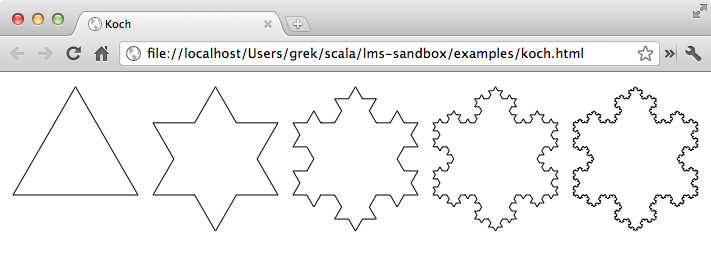
\includegraphics[scale=0.4]{koch-browser}
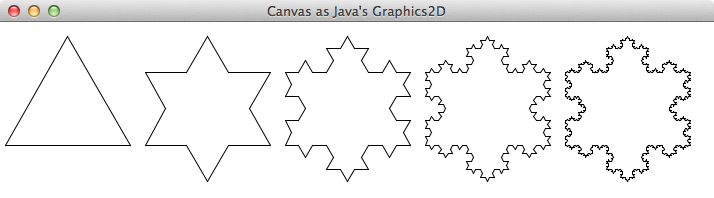
\includegraphics[scale=0.4]{koch-java2d}
\caption{Snowflakes rendered using HTML5 Canvas and Java's 2D}
\label{fig:snowflakes}
\end{figure}

HTML5 Canvas is a standard that is not implemented by all browsers yet so a fall-back mechanism is needed to support users of older browsers. This can be achieved through the trivial embedding by drawing using Java's 2D API, saving the result as an image and sending it to the browser. The decision to either generate a JavaScript snippet that draws on canvas and send it to the browser, or render the image on the server can be made at runtime (e.g. after inspecting information about the client's browser). In the case of rendering on the server-side, one can store computation that renders an image using Java's graphics 2D in a hash map and send back to the client the key as an url for an image. When a browser makes a second request, computation can be restored from the hash map, executed and the result sent back to the browser. All of that is possible because the computation itself is expressed against an abstract DSL API so we can swap implementations to either generate JavaScript or run the computation at the server side. Moreover, our DSL is just a library and computations are expressed as first-class values in a host language so they can be passed around the server program, stored in a hash map, etc.

A drawback of the trivial embedding is that the virtualization overhead is incurred each time the program is evaluated. To avoid this, we could generate Scala code in the same way as we now generate JavaScript code, relying on a mechanism to incorporate the generated Scala code into the rest of the program. In fact, this approach is taken by the Delite framework.

%- DOM Canvas Koch example: generate both client-side code or desktop widget

\section{Modularity Interlude}\label{sec:modularity}

The design of our DSL supports modularity at many levels. We use
Scala's traits heavily to allow our DSL to be assembled from and
extended with components~\cite{components-scala}.

For example, the feature to escape into dynamic typing is implemented
as an independent component that can be mixed and matched with
others. Similarly, users specify external APIs as components. The
separation between the interface level and the implementation level is
also done by having distinct components for each level. This allows
the same DSL program to be interpreted in multiple ways, as has been
shown with the trivial embedding to Scala.

As the features available in a DSL program are specified by composing
components, it is possible to use this mechanism to enforce that a
subprogram only uses a restricted set of features. For example, worker
threads in JavaScript (``WebWorkers'') are not allowed to manipulate
the DOM. This can be enforced by not mixing in the DOM component in
the subprogram for a worker thread.

The code generation level is assembled from components as in the
interface and implementation levels. Furthermore, optimizations in
code generation can be implemented as optional components to be mixed
in.

\section{Reification of Objects}\label{sec:reification}

By exploiting staging, the generated code can remain simple and
relatively unstructured as many of the high-level constructs can be
evaluated away at staging time. However, it is sometimes useful to be
able to reify more complex structures. For example, APIs sometimes
expect arguments or return results as object literals. Therefore, we
support a few type-safe ways to create more complex staged structures,
which we explain below.

\subsection{Functions}\label{sec:functions}

A function in the host language acting on reified types has type:
\code{Rep[A] => Rep[B]}. For example, the function \code{inc} has type
\code{Rep[Int] => Rep[Int]}:
\begin{lstlisting}
val inc = (x: Rep[Int]) => x + 1
\end{lstlisting}

Invoking such a function at staging time simply inlines the call:
\code{inc(4*x)} results in \code{4*x + 1}. This is useful and nice,
because it removes abstraction overhead from the generated
code.

We also want the ability to treat functions as first-class staged
values, since JavaScript supports them. In order to do this, we
provide a higher-order function \code{fun} which takes a function of
type \code{Rep[A] => Rep[B]} and converts\footnote{We refer the reader
  to ~\cite{lms} for implementation details} it to a staged function
of type \code{Rep[A => B]}. For example, if we define \code{inc} in
the following way, its type is \code{Rep[Int => Int]}:
\begin{lstlisting}
val inc = fun { (x: Rep[Int]) => x + 1 }
\end{lstlisting}
Calling \code{inc(4*x)} results in an \code{Apply} IR node. We
actually generate JavaScript code for the staged \code{inc} function,
while we didn't for the unstaged one, since it's inlined at every call
site during staging. The generated code looks roughly like the
following:
\begin{lstlisting}[language=JavaScript]
var inc = function(a) {
  return a+1
}
inc(4*x)
\end{lstlisting}

First-class functions are widely used in JavaScript. One particular
common case is for callback-driven programming. Therefore, staged
functions are important to interface with existing libraries. They
will also play a crucial role in section~\ref{sec:cps}, where we
abstract over callback-driven programming.

\subsection{Typed Object Literals}\label{sec:object-literals}

Our DSL provides typed immutable object literals to represent
JavaScript object literals. As an example:
\begin{lstlisting}
val o = new JSLiteral {
  val a = 1
  val b = a + 1
}
\end{lstlisting}
\code{o} has type \code{Rep[JSLiteral \{val a: Int; val b: Int\}]}. All
the fields of \code{o} are \code{Rep}s, so \code{o.a} has type
\code{Rep[Int]}. The translation to JavaScript is straightforward:
\begin{lstlisting}
var o = { a : 1, b : 2 }
\end{lstlisting}
This straightforward translation makes it possible to pass the typed
object literals of our DSL to JavaScript functions which expects
object literals, such as \code{JSON.stringify} or jQuery's \code{css}.

As for implementation, notice that the type of a \code{new JSLiteral
  \{...\}} expression is not \code{JSLiteral \{...\}} but
\code{Rep[JSLiteral \{...\}]}. This is achieved with support from the
Scala-Virtualized compiler. \code{JSLiteral} inherits from a special
trait, which indicates its \code{new} expressions should be
reified. So the \code{new} expression is turned into a method call,
with information about all the field definitions. A complication is
that a field definition might reference another field being defined
(such as \code{b} being defined in terms of \code{a} in the example
above). So each definition is represented by its name and a {\it
  function} which takes a self type for the object literal. These
definition functions are evaluated in an order which allows the self
references to be resolved.

\subsection{Classes}\label{sec:reified-classes}
Our DSL also supports reified classes. For convenience, these are
defined as traits, use the \code{repProxy} mechanism underlying typed
APIs and are also implemented using reflection. The translation to
JavaScript, based on constructors and prototypes, is
straightforward. Through the trivial embedding, classes implemented in
our DSL can be used on both the server and client sides.

% contribution to LMS, completeness
%- JS Literals: intuitive translation to JS as useful JSON-like objects, static typing
%- mice example: shows use of JSLiterals + API gluing (create abstractions that you need, not necessarily exactly matching the underlying JS API)
%- reification of traits: mutability, inheritance

\section{CPS Transformation for Asynchronous Code Patterns}\label{sec:cps}
  A callback-driven programming style is pervasive in JavaScript programs. Because of lack of thread support, callbacks are used for I/O, scheduling and event-handling. For example, in an Ajax call, one has to provide a callback that will be called once the requested data arrives from the server. This style of programming is known to be unwieldy in more complicated scenarios. To give a specific example, let's consider a scenario where we have an array of Twitter account names and we want to ask Twitter for the latest tweets of each account. Once we obtain the tweets of all users, we would like to log that fact in a console.

We'll implement this program both in JavaScript and in our DSL. Let's start by implementing logic that fetches tweets for a single user by using the jQuery library for Ajax calls (listings~\ref{code:js:twitter_fetch}~\&~\ref{code:twitter_fetch}).

\lstset{basicstyle=\ttfamily\scriptsize}
\begin{figure}
\setlength{\columnseprule}{0.5pt}
\begin{changemargin}{-1.5cm}{-1.5cm}
\begin{multicols}{2}
\lstinputlisting[language=JavaScript,caption=Fetching tweets in JavaScript,label=code:js:twitter_fetch]{fetchTweets.js}
\lstinputlisting[escapechar=|,caption=Fetching tweets in DSL,label=code:twitter_fetch]{fetchTweets.scala}
\end{multicols}
\end{changemargin}
\end{figure}

Note that JavaScript version takes a callback as second argument that will be used to process the fetched tweets. We provide the rest of the logic that iterates over an array of users and makes Ajax requests (listings~\ref{code:js:twitter_example}~\&~\ref{code:twitter_example}).

\begin{figure}
\begin{changemargin}{-0.7cm}{-0.7cm}
\setlength{\columnseprule}{0.5pt}
\begin{multicols}{2}
\lstinputlisting[language=JavaScript,caption=Twitter example in JavaScript,label=code:js:twitter_example]{twitter.js}
\lstinputlisting[escapechar=|,caption=Twitter example in DSL,label=code:twitter_example]{twitter.scala}
\end{multicols}
\end{changemargin}
\end{figure}

\lstset{basicstyle=\ttfamily}

Because of the inverted control flow of callbacks, synchronization between callbacks has to be handled manually. Also, the inverted control flow leads to a code structure that is distant from the programmer's intent. Notice that the in JavaScript version, the call to console that prints ``done" is put inside of the foreach loop. If it was put it after the loop, we would get ``done'' printed \emph{before} any Ajax call has been made leading to counterintuitive behaviour.

As an alternative to the callback-driven programming style, one can use an explicit monadic style, possibly sugared by a Haskell-like ``do''-notation. However, this requires rewriting possibly large parts of a program into monadic style when a single async operation is added. Another possibility is to automatically transform the program into continuation passing style (CPS), enabling the programmer to express the algorithm in a straightforward, sequential way and creating all the necessary callbacks and book-keeping code automatically. Links~\cite{links} uses this approach. However, a whole-program CPS transformation can cause performance degradation, code size blow-up, and stack overflows. In addition, it is not clear how to interact with existing non-CPS libraries as the whole program needs to adhere to the CPS style. We suggest using a {\it selective} CPS transformation, which precisely identifies what needs to be CPS transformed.

In fact, the Scala compiler already does selective, \code{@suspendable} type-annotation-driven CPS transformations of Scala programs~\cite{cps-scala,danvy90,danvy92}. We show how this mechanism can be used for transforming our DSL code before staging and stripping out most CPS abstractions at staging time. The generated JavaScript code doesn't have any CPS-specific code but is written in CPS-style by use of JavaScript anonymous functions.

Our implementation to support continuations is an example of an interesting technique of applying selective cps
transformation to embedded DSLs by means of a deep linguistic reuse, exploiting a host language feature to
implement the corresponding DSL feature without (much) additional work. An interesting insight is that CPS
transforming a program generator allows it to generate code that is in CPS.

\subsection{CPS in Scala}
Before presenting how CPS transformations are used in our DSL, let's consider a typical situation where CPS rewrites act on Scala programs.

As an example, we'll consider a \code{sleep} method implemented in non-blocking, asynchronous style. This is useful, for example, when using \code{ThreadPool}s as no thread is being blocked during the sleep period. Let's see how our \code{sleep} method written in CPS can be used:

\begin{lstlisting}
def foo() = {
  sleep(1000)
  println("Called foo")
}
reset {
  println("look, Ma ...")
  foo()
  sleep(1000)
  println(" no threads!")
}
\end{lstlisting}

The \code{reset} delimits the scope of CPS rewrite. Let's see how the rewrite itself looks like:

\begin{lstlisting}
def foo(): ControlContext = {
  sleep(1000).map((tmp1: Unit) => println("Called foo"))
}
reset {
  println("look, Ma ...")
  foo().flatMap((tmp2: Unit) =>
    sleep(1000).map((tmp3: Unit) => println(" no threads!"))
  )
}
\end{lstlisting}

There are a few things worth noting here. First, the return type of
\code{foo} method is rewritten to be
\code{ControlContext}.\footnote{The \code{ControlContext} class
  implements the continuation monad and is provided by Scala's
  standard library. \code{ControlContext[A,B,C]} is similar to C\#'s
  \code{Task<T>}, but more general. In our discussion, we omit the
  type parameters for simplicity.} This is due to the fact that
\code{sleep} is used in the body of \code{foo}. Also, note that the
code to be executed after sleeping is captured as a continuation
(anynomous function) and passed to the \code{ControlContext} through a
call of the \code{map} method. The body of the \code{reset} block is
rewritten in a similar vein.

Now, let's have a closer look how \code{sleep} itself is implemented:

\begin{lstlisting}[label={code:cps_scala},caption={\code{sleep} implementation}]
import java.util.{Timer,TimerTask}
val timer = new Timer
def sleep(delay: Int): Unit @suspendable = shift { k =>
  val task = new TimerTask { def run() = k() }
  timer.schedule(task, delay.toLong)
}
\end{lstlisting}

Notice the \code{@suspendable} type annotation attached to \code{sleep}'s return type \code{Unit}. The \code{@suspendable} annotation means that the \code{sleep} method can be used in a side-effecting continuation context. In the definition of the \code{sleep} method, we use Java's \code{Timer} and \code{TimerTask} abstractions for asynchronous, delayed task execution. The \code{TimerTask} interface has one method, \code{run}, that will be executed after a specified period of time. The \code{shift} control abstraction allows us to capture the continuation as a first-class value and then use it in the body of the \code{run} method. Both the \code{reset} and \code{shift} control abstractions are described in detail in~\cite{danvy90}.

After the CPS transformation, the code presented above becomes
\begin{lstlisting}
def sleep(time: Int): ControlContext =
  shiftR { k =>
    val task = new TimerTask { def run() = k() }
    timer.schedule(task, delay.toLong)
  }
\end{lstlisting}

After the rewriting, all CPS-related type annotations are dropped and use of the \code{ControlContext} class that supports continuation passing is introduced. The \code{shiftR} method is an internal method that takes a block (which itself is a function) and wraps it in \code{ControlContext} structure.

\subsection{CPS and Staging}
Let's write the example from listing~\ref{code:cps_scala} in our DSL. We need to define \code{sleep} to use JavaScript's \code{setTimeout}
\footnote{The \code{setTimeout} function asynchronously executes a function passed as argument after a specified delay.}
as a replacement for the \code{Timer} abstraction.
\begin{lstlisting}
def sleep(delay: Rep[Int]) = shift { k: (Rep[Unit]=>Rep[Unit]) =>
  window.setTimeout(fun(k), delay)
}
\end{lstlisting}

The \code{setTimeout} method expects an argument of type \code{Rep[Unit=>Unit]} which denotes a \emph{representation} of a function of type \code{Unit=>Unit}. The \code{shift} method offers us a function of type \code{Rep[Unit] => Rep[Unit]}, so we need to reify it to obtain the desired representation. The reification is achieved by the \code{fun} function (described in \ref{sec:functions}) provided by our framework and performed at staging time.

It's important to note that reification preserves function composition. Specifically, let \code{f: Rep[A] => Rep[B]} and \code{g: Rep[B] => Rep[C]} then {\tt\small fun(g compose f) == (fun(g) compose fun(f))} where we consider two reified functions to be equal if they yield the same observable effects at runtime. That property of function reification is at the core of reusing the continuation monad in our DSL. Thanks to the fact that the continuation monad composes functions, we can just insert reification at some places (like in a \code{sleep}) and make sure that we reify \emph{effects} of the continuation monad without the need to reify the monad itself.

\subsection{CPS for Suspendable Traversals}
We need to be able to suspend our execution while traversing an array in order to implement functionality from listing~\ref{code:twitter_example}. Let's consider a simplified example where we want to iterate over an array and sleep during each iteration. We present both code written in JavaScript and our DSL that achieves that (listings~\ref{code:js:sleep_iter}~\&~\ref{code:sleep_iter}).
\begin{figure}
\lstset{basicstyle=\ttfamily\scriptsize}
\begin{changemargin}{-0.7cm}{-0.7cm}
\setlength{\columnseprule}{0.5pt}
\begin{multicols}{2}
\begin{lstlisting}[caption=JavaScript,label=code:js:sleep_iter]
var xs = [1, 2, 3]
var i = 0
var msg = null
function f1() {
  if (i < xs.length) {
    window.setTimeout(f2, xs[i]*1000)
    msg = xs[i]
    i++
  } else {
    console.log("done")
  }
}
function f2() {
  console.log(msg)
  f1()
}
f1()
\end{lstlisting}
\begin{lstlisting}[escapechar=|,caption=DSL,label=code:sleep_iter]
val xs = array(1, 2, 3)
// shorthand for xs.suspendable.foreach
for (x <- xs.suspendable) {
  sleep(x * 1000)
  console.log(String.valueOf(x))
}
log("done")








|$\quad$|
\end{lstlisting}
\end{multicols}
\end{changemargin}
\lstset{basicstyle=\ttfamily}
\end{figure}

Both programs, when executed, will print the following to the JavaScript console:
\begin{lstlisting}
//pause for 1s
1
//pause for 2s
2
//pause for 3s
3
done
\end{lstlisting}

In the DSL code, we use a \code{suspendable} variant of arrays, which is achieved through an implicit conversion from regular arrays:
\begin{lstlisting}
implicit def richArray(xs: Rep[Array[A]]) = new {
  def suspendable: SArrayOps[A] = new SArrayOps[A](xs)
}
\end{lstlisting}
The idea behind \code{suspendable} arrays is that iteration over them can be suspended. We'll have a closer look at how to achieve that with the help of CPS. The \code{suspendable} method returns a new instance of the \code{SArrayOps} class defined here:

\begin{lstlisting}[caption=Suspendable foreach,label=code:suspendable_foreach]
class SArrayOps(xs: Rep[Array[A]]) {
  def foreach(yld: Rep[A] => Rep[Unit] @suspendable):
    Rep[Unit] @suspendable = {
      var i = 0
      suspendableWhile(i < xs.length) { yld(xs(i)); i += 1 }
    }
}
\end{lstlisting}
Note that one cannot use while loops in CPS but we can simulate them
with recursive functions. Let's see how a regular while loop can be
simulated with a recursive function with call-by-name parameters:
\begin{lstlisting}
def recursiveWhile(cond: => Boolean)(body: => Unit): Unit = {
  def rec = () => if (cond) { body; rec() } else {}
  rec()
}
\end{lstlisting}

By adding CPS-related declarations and control abstractions, we implement \code{suspendableWhile}:

\begin{lstlisting}
def suspendableWhile(cond: => Rep[Boolean])(
  body: => Rep[Unit] @suspendable): Rep[Unit] @suspendable =
  shift { k =>
    def rec = fun { () =>
      if (cond) reset { body; rec() } else { k() }
    }
    rec()
  }
\end{lstlisting}

\subsection{Defining the Ajax API}

With the abstractions for suspendable loops and traversals at hand,
what remains to complete the Twitter example from the beginning of the section
is the actual Ajax request/response cycle.

The Ajax interface component provides a type \code{Request} that captures the 
request structure expected by the underlying JavaScript/jQuery implementation and the
necessary object and method definitions to enable the use of \code{ajax.get} in user
code:
\begin{lstlisting}
trait Ajax extends JS with CPS {
  type Request = JSLiteral {
    val url: String
    val `type`: String
    val dataType: String
    val data: JSLiteral
  }
  type Response = Any
  object ajax {
    def get(request: Rep[Request]) = ajax_get(request)
  }
  def ajax_get(request: Rep[Request]): Rep[Response] @suspendable
}
\end{lstlisting}

Notice that the \code{Request} type is flexible enough to support an arbitrary object literal type for the \code{data} field through subtyping. The \code{Response} type alias points at \code{Any} which means that it is the user's responsibility to either use \code{dynamic} or perform an explicit cast to the expected data type.

The corresponding implementation component implements \code{ajax_get} to capture a continuation, reify it as a staged function using \code{fun} and store it in an \code{AjaxGet} IR node. 
\begin{lstlisting}
trait AjaxExp extends JSExp with Ajax {
  case class AjaxGet(request: Rep[Request],
    success: Rep[Response => Unit]) extends Def[Unit]
  def ajax_get(request: Rep[Request]): Rep[Response] @suspendable = 
    shift { k =>
      reflectEffect(AjaxGet(request, fun(k)))
    }
}
\end{lstlisting}

During code generation, we emit code to attach the captured continuation as a callback function in the \code{success} field of the request object:
\begin{lstlisting}
trait GenAjax extends JSGenBase {
  val IR: AjaxExp
  import IR._
  override def emitNode(sym: Sym[Any], rhs: Def[Any])(
    implicit stream: PrintWriter) = rhs match {
      case AjaxGet(req, succ) => 
        stream.println(quote(req) + ".success = " + quote(succ)) 
        emitValDef(sym, "jQuery.ajax(" + quote(req) + ")")
    case _ => super.emitNode(sym, rhs)
  }
}
\end{lstlisting}

It's interesting to note that, since the request already has the right structure for the \code{jQuery.ajax} function, we can simply pass it to the framework-provided \code{quote} method, which knows how to generate JavaScript representations of any \code{JSLiteral}.

The Ajax component completes the functionality required to run the Twitter example with one caveat:
The outer loop in listing~\ref{code:twitter_example} uses \code{parSuspendable} to traverse arrays instead of the \code{suspendable} traversal variant we have defined in listing~\ref{code:suspendable_foreach}. 

In fact, if we change the code to use \code{suspendable} instead of \code{parSuspendable} and run the generated JavaScript program, we'll get following output printed to the JavaScript console:
\begin{lstlisting}
fetching gkossakowski
finished fetching gkossakowski
fetched [...]
fetched [...]
fetching odersky
finished fetching odersky
fetched [...]
fetched [...]
fetching adriaanm
finished fetching adriaanm
fetched [...]
fetched [...]
done
\end{lstlisting}

Notice that all Ajax requests were done sequentially. Specifically,
there was just one Ajax request active at a given time; when the
callback to process one request is called, it would resume the
continuation to start another request, and so on. In many cases this
is exactly the desired behavior, however, we will most likely
want to perform our Ajax request in parallel.

\subsection{CPS for Parallelism}
The goal of this section is to implement a parallel variant of the
\code{foreach} method from listing~\ref{code:suspendable_foreach}. We'll start 
with defining a few primitives like futures and dataflow cells. 
Let's start with cells, which we
decide to define in JavaScript, as another example of
integrating external libraries with our DSL:

\begin{lstlisting}[language=JavaScript,caption=JavaScript-based implementation of a non-blocking Cell]
function Cell() {
  this.value = undefined
  this.isDefined = false
  this.queue = []
  this.get = function (k) {
    if (this.isDefined) {
      k(this.value)
    } else {
      this.queue.push(k)
    }
  }
  this.set = function (v) {
    if (this.isDefined) {
      throw "can't set value twice"
    } else {
      this.value = v
      this.isDefined = true
      this.queue.forEach(function (f) { 
        f(v) //non-trivial spawn could be used here
      })
    }
  }
}
\end{lstlisting}

A cell object allows us to track dependencies between values. Whenever the \code{get} method is called and the value is not in the cell yet, the continuation will be added to a queue so it can be suspended until the value arrives. The \code{set} method takes care of resuming queued continuations. We expose \code{Cell} as an external library using our typed API mechanism and we use it for implementing an abstraction for futures.

\begin{lstlisting}
def createCell(): Rep[Cell[A]]
trait Cell[A]
trait CellOps[A] {
  def get(k: Rep[A => Unit]): Rep[Unit]
  def set(v: Rep[A]): Rep[Unit]
}
implicit def repToCellOps(x: Rep[Cell[A]]): CellOps[A] =
  repProxy[Cell[A],CellOps[A]](x)

def spawn(body: => Rep[Unit] @suspendable): Rep[Unit] = {
  reset(body) //non-trivial implementation uses
              //trampolining to prevent stack overflows
}
def future(body: => Rep[A] @suspendable) = {
  val cell = createCell[A]()
  spawn { cell.set(body) }
  cell
}
\end{lstlisting}

The last bit of general functionality we need is \code{RichCellOps} that ties \code{Cell}s and continuations together inside of our DSL.

\begin{lstlisting}
class RichCellOps(cell: Rep[Cell[A]]) {
  def apply() = shift { k: (Rep[A] => Rep[Unit]) =>
    cell.get(fun(k))
  }
}
implicit def richCellOps(x: Rep[Cell[A]]): RichCell[A] =
  new RichCellOps(x)
\end{lstlisting}

It's worth noting that \code{RichCellOps} is not reified so it will be dropped at staging time and its method will get inlined whenever used. Also, it contains CPS-specific code that allows us to capture the continuation. The \code{fun} function reifies the captured continuation.

We are ready to present the parallel version of \code{foreach} defined in listing \ref{code:suspendable_foreach}.

\begin{lstlisting}
def foreach(yld: Rep[A] => Rep[Unit] @suspendable):
  Rep[Unit] @suspendable = {
    val futures = xs.map(x => future(yld(x)))
    futures.suspendable.foreach(_.apply())
  }
\end{lstlisting}

We instantiate each future separately so they can be executed in parallel. As a second step we make sure that all futures are evaluated before we leave the \code{foreach} method by forcing evaluation of each future and ``waiting'' for its completion. Thanks to CPS transformations, all of that will be implemented in a non-blocking style.

The only difference between the parallel and serial versions of the Twitter example~\ref{code:twitter_example} is the use of \code{parSuspendable} instead of \code{suspendable} so the parallel implementation of the \code{foreach} method is used. The rest of the code stays the same. It's easy to switch between both versions, and users are free to make their choice according to their needs and performance requirements.


%Parallelism doesn't come for free as it involves more CPS rewritings and involves indirections introduced by our abstractions. However, since it's easy to switch between both versions, users are free to make those choices according to their needs and performance requirements.

\section{Evaluation}\label{sec:eval}

We've implemented our DSL in Scala.\footnote{The code can be found at
  \url{http://github.com/js-scala}} We used our DSL to
develop a few web applications, which are simple but not
trivial. First, we implemented a few drawing examples like the
snowflakes of figure~\ref{fig:snowflakes}. We extended the Twitter
example from section~\ref{sec:cps}, which presents the latest tweets
from selected users in an interactive way. In order to do so, we
incorporated a useful subset of the DOM API and jQuery library using our
typed APIs.

Also, we integrated our DSL with an existing web framework, Play 2.0.\footnote{\url{http://www.playframework.org}}
Our DSL can be used to define Play form validators that are executed on both the client and server sides.
We managed to achieve that without deep changes to how the framework works internally proving that our
DSL can be used as a library.

\begin{wrapfigure}{r}{5cm}
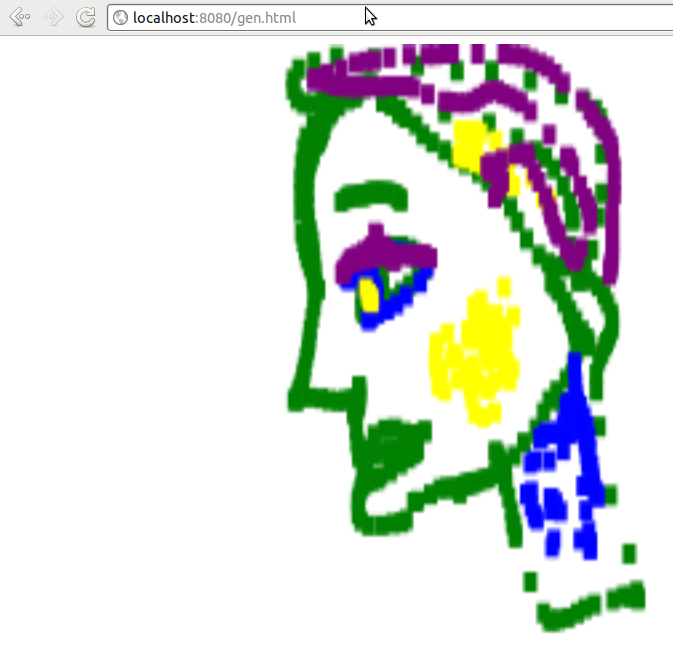
\includegraphics[scale=0.2]{drawing}
\end{wrapfigure}
Finally, we developed a collaborative drawing application, which
includes a server-side component (implemented using the Jetty web
server). We use web sockets to communicate between the server and
clients. Each client transmits drawing commands to the server, which
broadcasts them to all the clients. When a new client joins, the
server sends the complete drawing history to the new client, and the
client reconstructs the image by playing the commands. A very
simple improvement is to make the server execute the drawing
commands as well, and keep an up-to-date bitmap of the drawing -- this
can easily be achieved by using the trivial embedding described in
section~\ref{sec:trivial-embedding}. New clients then just obtain the
bitmap instead of replaying the history, which is potentially large.

\section{Conclusion}\label{sec:conclusion}

In this paper, we have shown how to embed a JavaScript DSL in Scala
using LMS. A recurring theme of our approach is to exploit the
features of the host language to enhance the DSL with minimal
effort. Moreover, through staging, we can use many abstractions at the
code-generation stage, without complexity and performance overhead in
the generated code. We believe this approach addresses some important
challenges of developing rich web applications.

\section{Acknowledgments}
We thank Adriaan Moors for maintaining the Scala-Virtualized compiler, adding our feature requests, fixing our reported bugs, and for insightful discussions.

\bibliographystyle{abbrv}
\bibliography{refs,ppl}


\end{document}
